
\documentclass{article}
\usepackage{latexsym}
\usepackage{url}
\usepackage{hyperref}
\hypersetup{colorlinks=true}
\usepackage{graphicx}

\begin{document}

\title{Artifficial Intelligence Project}
\author{Mitre Flavia Antonia }
\date{\today}

\maketitle

\begin{tabbing}
\indent{Second Year}\\
\indent{Group: C.E.N. 2.1}\\
\indent{Lecturer:} \href{http://software.ucv.ro/~cbadica}{Costin B\u{a}dic\u{a}} \\
\indent{Teaching assistant:}  Ionu\c{t} Murare\c{t}u \\


\end{tabbing}
\pagebreak


\section{Problem statement}
P1 Suppose two friends live in different cities on a map, such as the Romania
map shown in Figure 2. On every turn, we can simultaneously move each
friend to a neighboring city on the map. The amount of time needed to
move from city i to neighbor j is equal to the road distance d(i, j) between
the cities, but on each turn the friend that arrives first must wait until the
other one arrives (and calls the first on his/her cell phone) before the next
turn can begin. We want the two friends to meet as quickly as possible.


An example of how the map for this problem should look:
\linebreak
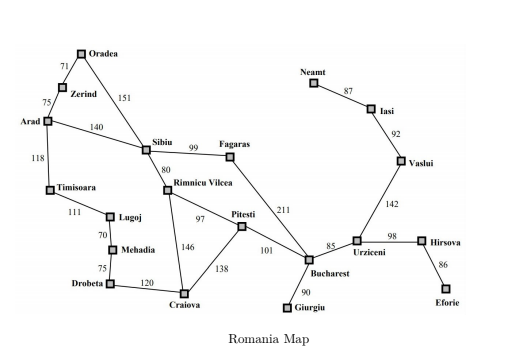
\includegraphics[scale=0.5]{romania.png}
 
 \linebreak
 
a. Write a detailed formulation for this search problem.

b. Identify a search algorithm for this task and explain your choice.\\
\linebreak

The input will be given as:
	
	\begin{enumerate}	\item Two text files containing the number of cities that can be travelled, and the matrixes of costs each number on a line.
		\end{enumerate}
		\pagebreak
How I computed the hash
value to obtain the problem's number:

Made the sum of the ASCII codes of all the characters in my last and 1st first name.
\\
\\
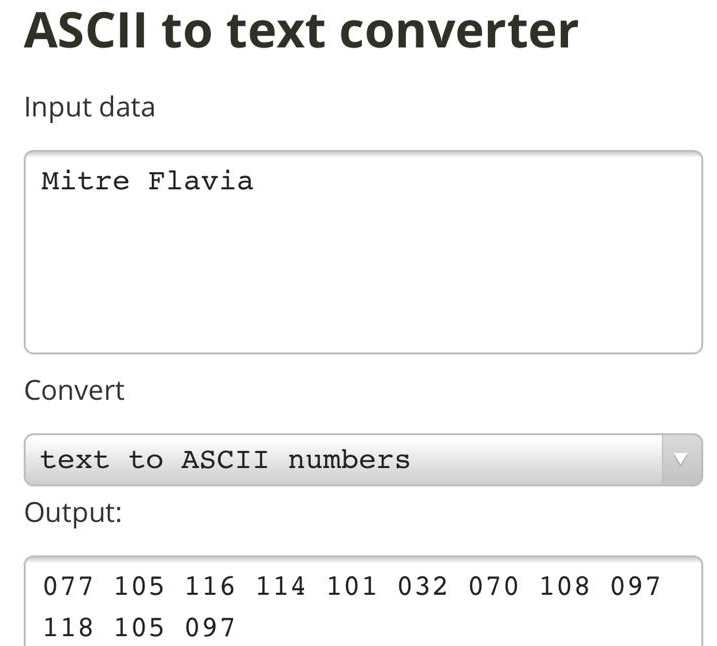
\includegraphics[scale=0.35]{asciiConvName.png}
\\
\\

The sum is equal to 1140 (77 + 105 + 116 + 114 + 101 + 32 + 70 + 108 + 97 + 118 + 105 + 97).
The final result that gives the number of the problem is: one plus the sum modulo 4 (1 + (1140 modulo 4) = 1 + 0 = 1).
 	\pagebreak
\section{Application design and algorithms}

\begin{itemize}
    
\item
The program is based on using algorithms. The correct approach for this problem is solving using Dynamic Programming.\end{itemize}
\begin{itemize}
  \item The application contains a P1.c file.
 
  \end{itemize}
  The main function is represented by :
  \begin{itemize}
  \item Initializing the maximum cost with 0.
  \end{itemize}
  \begin{itemize}
  \item The call of the function that reads the input from a file, for the first travel:  {takeInput(0)}.
  \end{itemize}
  \begin{itemize}
  \item Printing the path for the first travel.
  \end{itemize}
  \begin{itemize}
  \item The call of the function that calculates the minimum cost for the travel: {mincost(0,0)}.
  \end{itemize}
  \begin{itemize}
  \item The minimum cost for the first friend is printed here.
  \end{itemize}
  \begin{itemize}
  \item If the cost for the first friend is bigger than the maximum cost then the maximum cost takes its value. Then the variable "cost" becomes zero.
  \end{itemize}
  \begin{itemize}
  \item The call of the function that reads the input from a file, for the second travel:  {takeInput(1)}.
  \end{itemize}
  \begin{itemize}
  \item Printing the path for the second travel.
  \end{itemize}
  \begin{itemize}
  \item The call of the function that calculates the minimum cost for the travel: {mincost(0,1)}.
  \end{itemize}
  \begin{itemize}
  \item The minimum cost for the second friend is printed here.
  \end{itemize}
  \begin{itemize}
  \item If the cost for the second friend is bigger than the maximum cost then the maximum cost takes its value. 
  \end{itemize}
  
    \begin{figure}
\begin{center}
\begin{tabbing}

  TAKEINPUT($number$) \\
1. \indent \=$i \leftarrow 0$
 \\
2. \indent \=$nrchr \leftarrow 0$\\
3. {\bf if} \=$number$ = $0$
{\bf  do}\\

4. \indent \>Open file1 and read the data from file (number of cities and cost matrix).
\\
5.  else \\
6.  \indent \>Open file2 and read the data from file (number of cities and cost matrix).
\\

7. \indent   {\bf for} $i \leftarrow 0, nrchr-1, +1 $
{\bf  do}\\
8. \indent\> $aux \leftarrow m[i]$\\
9.  \indent\> $far[i] \leftarrow aux$\\
10. \indent\>$far[i] \leftarrow far[i]-48$\\
11. Close the file.\\
12. $n \leftarrow far[0] $\\
13. {\bf if} $r = 0$
{\bf do}\\
14.   \indent \> Write: "The number of villages is n"\\
15. \indent $k\leftarrow 1$\\
16. \indent   {\bf for} $i \leftarrow 0, n-1, +1 $
{\bf  do}\\
17.  \indent \>{\bf for} $j\leftarrow 0, n-1, +1 $
{\bf  do}\\
18.   \indent $ary[i][j] \leftarrow far[k]$\\
19.             \indent    $k \leftarrow k+1$\\
20. \indent $completed[i] \leftarrow 0$\\
21. \indent Write "The cost list is:"\\
22. \indent    {\bf for} $i \leftarrow 0, n-1, +1 $
{\bf  do}\\ 
23.   \indent  Write "enter"\\
24.   \indent \>{\bf for} $j\leftarrow 0, n-1, +1 $
{\bf  do}\\
25.  \indent     Write "tab ary[i][j]"\\
\end{tabbing}
\label{fig_alg_ex}
\caption{Function that reads the input data.}

\end{center}
\end{figure}

    \begin{figure}
\begin{center}
\begin{tabbing}
{LEAST}() \\
1. \indent              $nc \leftarrow 999$   \\
2. $min \leftarrow 999$ \\
3. \indent   {\bf for} $i \leftarrow 0, n-1, +1 $
{\bf  do}\\
4.    \indent  {\bf if} $ary[c][i]!=0 and completed[i]=0$
{\bf  do}\\
5.      \indent    {\bf if} $ary[c][i]+ary[i][c] < min$
{\bf  do}\\
6.  \indent  $min \leftarrow ary[i][0]+ary[c][i]$ \\
7.        \indent      $kmin \leftarrow ary[c][i]$ \\
8.        \indent      $nc \leftarrow i$ \\
9.       \indent   {\bf if} min!=999
{\bf  do}\\
10.       \indent $cost \leftarrow cost + kmin$ \\
11. \indent return nc \\
\end{tabbing}
\caption{Returning an int that is equal to the last i.}


\end{center}
\end{figure}

     \begin{figure}
\begin{center}
\begin{tabbing}
{MINCOST()} \\
1. $completed[city] \leftarrow 1$\\
2. \indent {\bf if} r = 0 
{\bf do}\\
3.  \indent   {\bf  if} $city = n-1$ {\bf do}\\
4.      \indent     $ fr \leftarrow 1$ \\
5.      \indent      Write $city+1$ \\
6.       \indent   return \\
7.  \indent else \\
8.      \indent Write $city+1 "\rightarrow"$ \\
9.      \indent $ncity \leftarrow least(city)$\\
10.  \indent {\bf if} $ncity = 999$ {\bf do}\\
11.   \indent      $ncity \leftarrow 0 $\\
12.  \indent $Write ncity+1$  \\
13.  \indent {\bf if} $city !=n-1$ {\bf do}\\
14.   \indent $cost \leftarrow cost + ary[city][ncity]$ \\
15. \indent return\\
16. \indent else \\
{\bf if} r = 0 {\bf do}\\
17.  \indent   {\bf  if} city = n-1 {\bf do}\\
18.   \indent   $   fr \leftarrow 1$ \\
19.   \indent      Write n-city \\
20. return \\
21. \indent else \\
22. \indent Write $n-city "\rightarrow"$ \\
23. \indent$ ncity \leftarrow least(city)$\\
24.  \indent {\bf if} $ncity$ = 999 {\bf do}\\
25.   \indent    $ncity \leftarrow 0$ \\
26.  \indent Write $ncity$+1  \\
27.  \indent {\bf if} $city$ !=n-1 {\bf do}\\
28.   \indent $cost \leftarrow cost$ + $ary[city][ncity]$ \\
29. \indent return\\
30.  \indent $mincost(ncity, r)$ \\

\end{tabbing}
\caption{This function computes the minimum cost.}
\label{fig_alg_ex3}

\end{center}
\end{figure}

     \begin{figure}
\begin{center}
\begin{tabbing}
  {MAIN}() \\
1. \indent $maxcost \leftarrow 0$ \\
2. \indent  takeInput(0) \\
3. \indent  Write "The Path from 1 to n is:"\\
4. \indent mincost(0,0) \\
5. \indent  Write "Minimum cost for the first friend is cost"\\
6. \indent $maxcost \leftarrow cost$ \\
7. \indent $cost \leftarrow 0$ \\
8. \indent  takeInput(1) \\
9. \indent  Write "The Path from n to 1 is:"\\
10. \indent mincost(0,1) \\
11. \indent Write:"Minimum cost for the second friend is cost"\\
12. \indent   {\bf  if} maxcost < cost {\bf do}\\
13. \indent $maxcost \leftarrow cost$ \\
14. \indent Write "The minimum cost for the two friends to meet is maxcost" \\
\end{tabbing}
\caption{The main function.}
\label{fig_alg_ex4}

\end{center}
\end{figure}

    \pagebreak
\section{Experimental Data}

In this section are a few non-trivial input tests and their outputs, and, also the execution time of every one of them.  

\begin{figure}[h!]
\centering
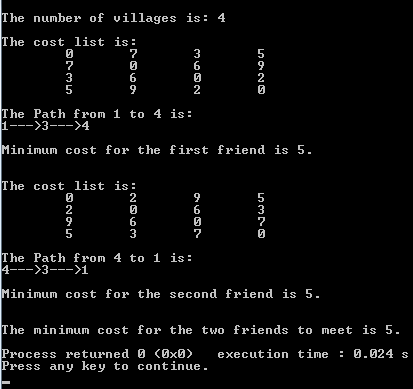
\includegraphics[scale=0.5]{secondexample.png}
\caption{Output for the first set of data.}
\label{fig:crypt}
\end{figure}
\begin{itemize}
    \item In this case the minimum costs for the two friends are the same. The time of execution is 0.024 seconds.\\
\end{itemize}
\begin{figure}[h!]
\centering
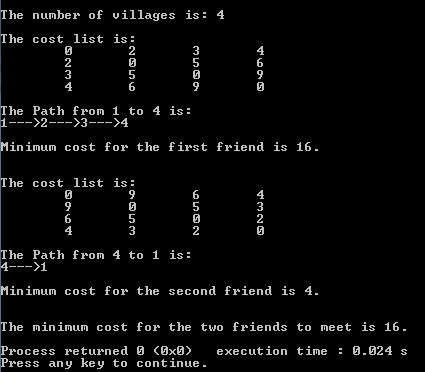
\includegraphics[scale=0.5]{firstexample.png}
\caption{Output for the second set of data.}
\label{fig:crypt}
\end{figure}

\begin{figure}[h!]
\centering
\label{fig:crypt}
\end{figure}
\begin{itemize}
    \item In this case the minimum costs for the two friends are different, we observe that the shortest path depends on the starting point as the minimum cost for the first friend is 4 and for the second friend is 16 . The time of execution is 0.024 seconds.\\
\end{itemize}


\pagebreak

\section{Conclusions}


This problem is an optimisation for the travelling salesman problem(TSP).
The travelling salesman problem asks the following question: "Given a list of cities and the distances between each pair of cities, what is the shortest possible route that visits each city and returns to the origin city?" It is an NP-hard problem in combinatorial optimization, important in operations research and theoretical computer science.\\
\linebreak
The greedy algorithm can be used to give a good but not optimal solution (it is an approximation to the optimal answer) in a reasonably short amount of time. The greedy algorithm heuristic says to pick whatever is currently the best next step regardless of whether that prevents (or even makes impossible) good steps later. It is a heuristic in that practice says it is a good enough solution, theory says there are better solutions (and even can tell how much better in some cases).\\
\linebreak

\pagebreak

\begin{thebibliography}{9}

\bibitem{latex}

\url{https://www.programiz.com/c-programming/examples/read-file}

\bibitem{latex}

\url{https://math.stackexchange.com/questions/2489528/traveling-salesman-problem-with-two-salesmen}
\bibitem{latex}

\url{https://en.wikipedia.org/wiki/Heuristic_(computer_science)}

\bibitem{latex}

\url{https://www.overleaf.com/learn/latex/Inserting_Images}

\end{thebibliography}
\pagebreak

 

    





\end{document}
